%!TeX root = ../main.tex

\section{Development}
\subsection{Training}
The images from the training set are loaded into a single image datastore. After that, a loop for each image is designed in order to:
\begin{enumerate}
\item Convert the image to grayscale;
\item Detect the SURF features (using the MATLAB function ``detectSURFFeatures'');
\item Extract the features (descriptors) using the function ``extractFeatures''. In this case they are represented as a vector of $64$ columns and $N$ rows;
\item Stack vertically the descriptors of each image in a single matrix.
\end{enumerate}
The result is a big matrix containing all the descriptors for each image in column. The autoencoder has been built using the function ``layerGraph'', which requires in input a vector ``layers'' containing the structure of the Neural Network. For this purpose, we chose the following three-layer structure:
\begin{itemize}
\item an input layer that receives features of dimension 64 (using \\ ``featureInputLayer(64)'');
\item two fully connected layers of dimension 6 and 64 (using ``fullyConnectedLayer(6)'' and ``fullyConnectedLayer(64)''), the second one having dimension 64 as will work as output layer;
\item a regression layer that will predict the reconstructed values (using \\ ``regressionLayer'').
\end{itemize}
After some testing, we found out that for the inside layer a dimension of $4$ was too strict (The reconstructed values were too compressed, i.e. too far from the input ones) while for $8$ they were too close to the input ones, so we opted for the compromise of $6$.
Regarding the training options, we decided to use an \emph{adam} (Adaptive Moment Estimation) optimizer and a maximum number of epochs of 2, since even after one epoch the training loss was pretty stable around $5\%$ (fig. \ref{fig:2epochs}).

\begin{figure}[H]
    \centering
    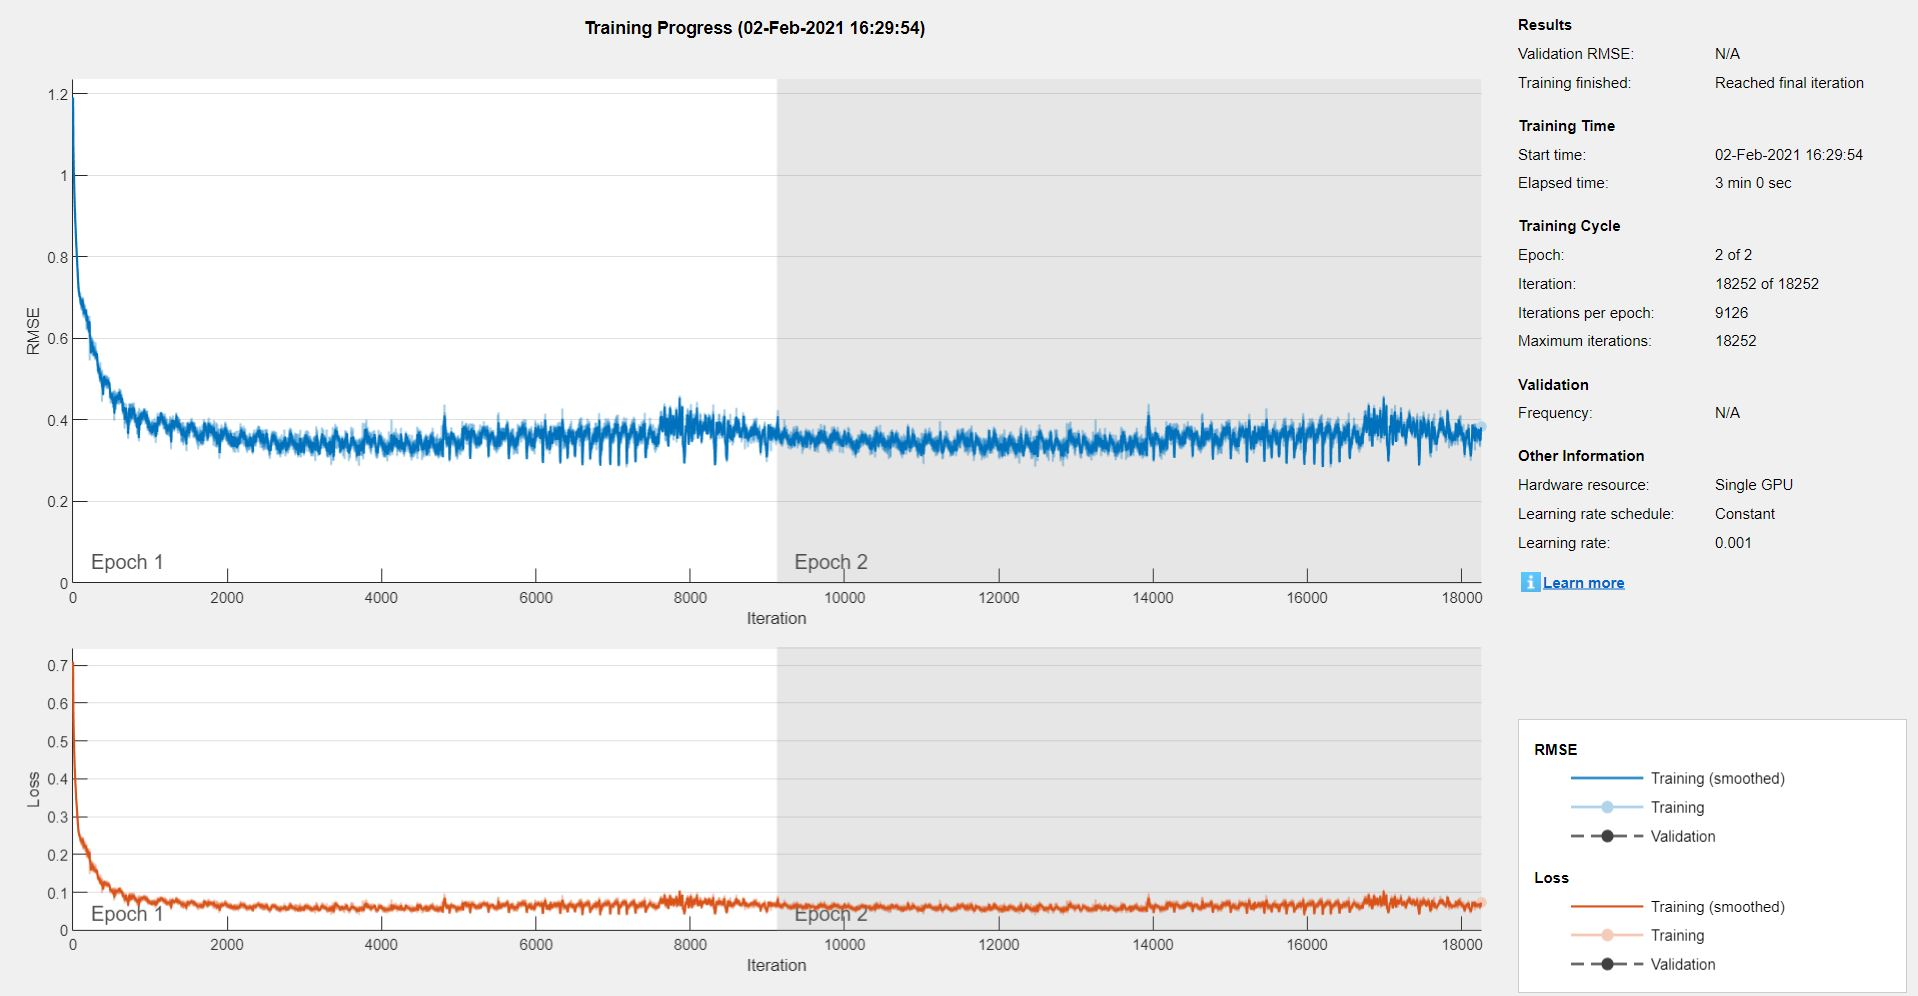
\includegraphics[width=\textwidth]{images/2EPOCHS.jpg}
    \caption{Training results after 2 epochs (18252 iterations).}
    \label{fig:2epochs}    
\end{figure}

The autoencoder is then succesfully trained (using the function ``trainNetwork'') in order to be ready to be used for the testing phase. A useful trick in order to fasten up the operation of testing and not doing everytime the training (which could require some time if the number of epochs is increased) is to save the workspace at the end of the training section and load it at the beginning of the testing one, so that everytime that section is called the autoencoder will remain trained just like it was the first time.

\subsection{Testing}
For the phase of testing the image datasets must be loaded separately (one for each building). To be clearer, this section simply called two functions, one for the features extraction, and one for the matchings calculations. This was done because COLMAP requires specific type of files in order to perform a reconstruction (will be better explained in sec. \ref{sec:COLMAP}).

\subsubsection{Function FEATURES} \label{sec:FEATURES}
This function aims to reconstruct the features of each image with the autoencoder and the original ones in a .txt file for each image in the form ``location\_x location\_y scale orientation'' followed by 128 zeros since COLMAP works with SIFT features, which are of that size.
The workflow of the function is the following:
\begin{itemize}
\item The path containing the features is cleaned from older files containing the features;
\item For each image in the image datastore considered, which is given in input along with the autoencoder:
\begin{enumerate}
\item The image is converted to grayscale;
\item The features are detected and then extracted like for the phase of training, only this time they won't be stacked in a single matrix but the features \textbf{extracted} are going to be fed into the autoencoder and be returned from the function while the \textbf{detected} ones are going to be divided in Location, Scale, Orientation in order to be printed in a .txt file of the form
\begin{align*}
& N\ 128 \\
& location_{x0} \ location_{y0} \ scale_0 \ orientation_0 \ 0\  ... (x128)\  0 \\
& location_{x1} \ location_{y1} \ scale_1 \ orientation_1 \ 0\  ... (x128)\  0 \\
& ... \\
& location_{xN} \ location_{yN} \ scale_N \ orientation_N \ 0\  ... (x128)\  0 \\
\end{align*}  
where $N$ is the number of features.
\end{enumerate} 
\end{itemize}

\subsubsection{Function MATCHINGS} \label{sec:MATCHINGS}
The function, given in input the image datastore considered and the features (compressed or not) matches the features of each couple of image $i,j$. To avoid repetitions ($i,j$ and $j,i$ have the same matchings) the MATLAB function ``matchFeatures'' is called for every $i,j$ for $i$ going from 1 to the last feature -1 and $j$ going from $i+1$ to the last feature. The matchings are all stacked in a single .txt file of the form:
\begin{align*}
& image0.jpg\ image1.jpg \\
& matching1_0\ matching1_1 \\
& matching2_0\ matching2_1 \\
& ... \\
& matchingN_0\ matchingN_1 \\
& \\
& image0.jpg\ image2.jpg \\
& matching1_0\ matching1_2 \\
& ...
\end{align*}  